\section{Method}
\label{sec:method}

% \begin{figure*}[t!]
%     \centering
%     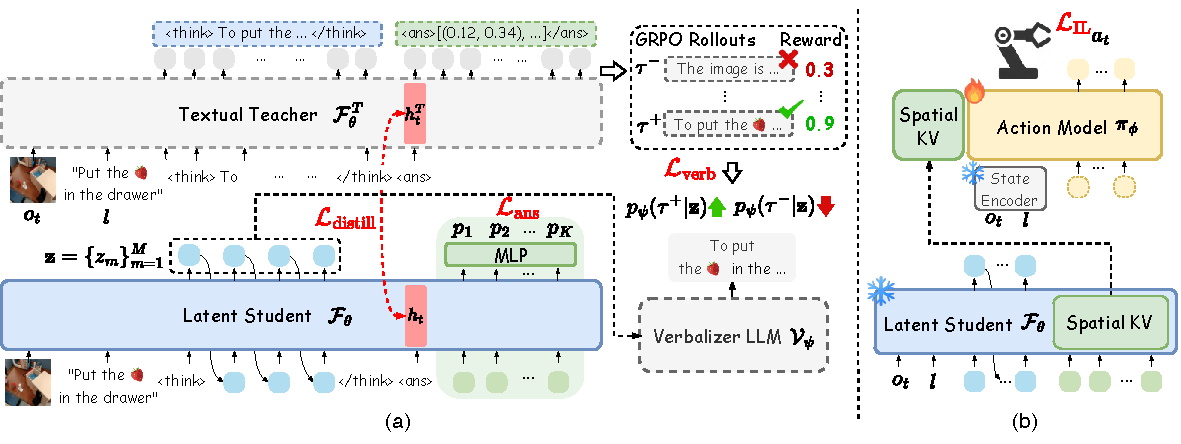
\includegraphics[width=0.95\linewidth]{figures/images/method.pdf}
%     \caption{\textbf{Overview of Fast-ThinkAct.} (a) Given observation $o_t$ and instruction $l$, the Textual Teacher VLM $\mathcal{F}_\theta^T$ generates explicit reasoning chains. The Latent Student VLM $\mathcal{F}_\theta$ distills these into compact latent tokens $\mathbf{z}$ guided by reward preferences. Verbalizer LLM $\mathcal{V}_\psi$ decodes latents to text for preference-based learning via $\mathcal{L}_{\text{verb}}$, while spatial tokens enable parallel visual trajectory prediction via $\mathcal{L}_{\text{ans}}$, ensuring latents are both verbalizable and grounded in visual planning. (b) Reasoning-Enhanced Policy Learning. The trained Latent Student $\mathcal{F}_\theta$ provides reasoning-infused multimodal guidance to the Action Model $\pi_\phi$ for executable action prediction.}
%     \label{fig:method}
%     % \vspace{-2mm}
% \end{figure*}

\begin{figure*}[t!]
    \centering
    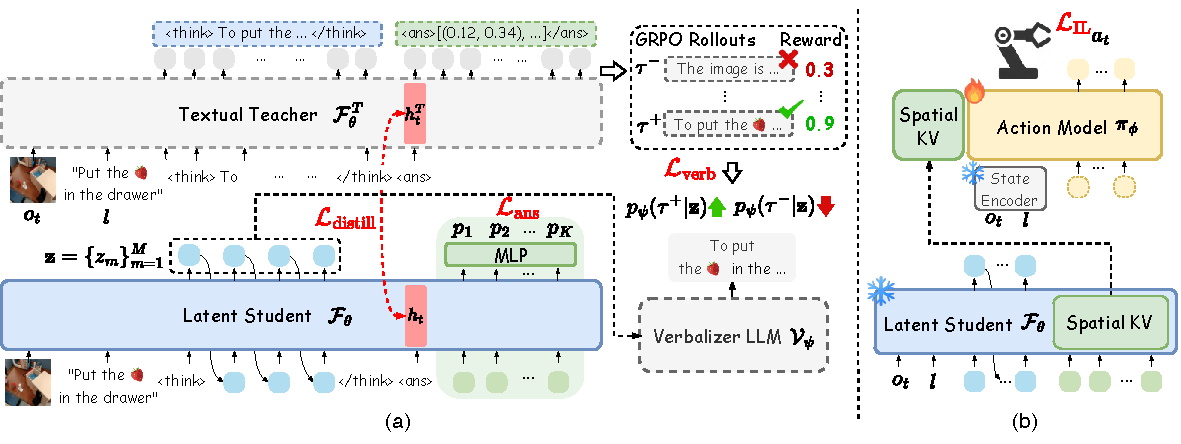
\includegraphics[width=1.0\linewidth]{figures/images/method.pdf}
    \caption{\textbf{Overview of Fast-ThinkAct.} (a) Given observation $o_t$ and instruction $l$, the Textual Teacher VLM $\mathcal{F}_\theta^T$ generates explicit reasoning chains. The Latent Student VLM $\mathcal{F}_\theta$ distills these into compact latent tokens $\mathbf{z}$ guided by reward preferences. Verbalizer LLM $\mathcal{V}_\psi$ decodes latents to text for preference-based learning via $\mathcal{L}_{\text{verb}}$, while $\mathcal{L}_{\text{distill}}$ transfers visual planning capability from teacher, and spatial tokens enable parallel visual trajectory prediction via $\mathcal{L}_{\text{ans}}$, ensuring latents are verbalizable and grounded in visual planning. (b) Reasoning-Enhanced Policy Learning. The Action Model $\pi_\phi$ is trained with $\mathcal{L}_{\text{IL}}$ while freezing the latent student $\mathcal{F}_\theta$ and state encoder.}
    \label{fig:method}
    % \vspace{-2mm}
\end{figure*}


\subsection{Problem Formulation}

We first define the setting and notations. At each timestep $t$, given a language instruction $l$, the model observes a visual input $o_t$ and generates an action chunk $a_t$, represented as a sequence of continuous robot control vectors (e.g., 7- or 14-DOF for single- or bimanual robots, respectively).

To address this problem, we propose \ours{}, an efficient reasoning framework that bridges high-level planning with low-level action execution. Our approach employs a VLM $\mathcal{F}_\theta$ to perform reasoning in \textit{continuous latent space}, integrated with an action model $\pi_\phi$ for executable action generation. Specifically, $\mathcal{F}_\theta$ processes observation-instruction pairs $(o_t, l)$ through latent chain-of-thought (CoT) reasoning to produce a compact visual plan latent $c_t$ that encapsulates the intended trajectory in visual space (Sec.~\ref{ssec:reasoning}). This $c_t$ subsequently guides $\pi_\phi$ to predict executable actions $a_t$ (Sec.~\ref{ssec:action}). By distilling reasoning into a continuous latent space rather than discrete text, \ours{} achieves significantly improved inference efficiency while enhancing action performance through better preservation of spatial and visual information.



\subsection{Efficient Embodied Reasoning}\label{ssec:reasoning}

To enable efficient embodied reasoning that meets the real-time requirements of embodied AI tasks, we aim to compress long textual CoTs into a compact set of continuous latent representations. However, compressing reasoning traces into latents is challenging, as there is no direct supervision signal in the latent space to guide what reasoning patterns should be encoded.

\subsubsection{Verbalizable Latent CoT by Reward Preferences}\label{sssec:verbalize}


To address this challenge, we propose to perform distillation in natural language space by introducing a verbalizer LLM that decodes latents into verbalizable reasoning. This approach grounds latent learning in an interpretable textual form, ensuring that the learned latents faithfully preserve the underlying reasoning structure. Since reasoning traces generated by the teacher model $\mathcal{F}_\theta^T$ exhibit varying quality, we adopt a preference-based learning framework that exploits reward signals from the teacher's GRPO training to guide the latent student $\mathcal{F}_\theta$ toward high-quality reasoning patterns while suppressing low-quality ones.


Specifically, we employ a teacher-student framework where a textual teacher model $\mathcal{F}_\theta^T$ first learns explicit reasoning through GRPO~\cite{shao2024deepseekmath} training by maximizing:
\begin{equation}
    \mathcal{J}_\text{GRPO}(\theta) = \mathbb{E}_{\tau\sim\mathcal{F}^T_\theta}\Big[ \min \big( r_\theta(\tau)A(\tau), \text{clip}(r_\theta(\tau), 1-\epsilon, 1+\epsilon )A(\tau) \big) \Big],
\end{equation}
where $\tau$ denotes a reasoning trace and $r_\theta(\tau) = \frac{\mathcal{F}^T_\theta(\tau)}{\mathcal{F}^T_{\text{old}}(\tau)}$ is the probability ratio. The advantage function for group rewards $\{ R_i \}_{i\in G(\tau)}$ is represented as:
\begin{equation}
     A(\tau)=\frac{R_\tau - \text{mean}(\{ R_i \}_{i\in G(\tau)})}{\text{std}(\{ R_i \}_{i\in G(\tau)})}.
\end{equation}

This training process produces textual CoTs with varying quality, where the advantage function $A(\tau)$ naturally serves as a quality indicator. To construct preference pairs for distillation, we select the highest and lowest advantage traces from each rollout group:
\begin{align}
\tau^+ = \arg\max_{\tau \in G} A(\tau) \text{ and } \tau^- = \arg\min_{\tau \in G} A(\tau).
\end{align}

Instead of generating textual tokens, the student model $\mathcal{F}_\theta$ performs latent reasoning by autoregressively generating $M$ continuous latent vectors $\mathbf{z} = \{z_m\}_{m=1}^M$ with $z_m \in \mathbb{R}^d$, where $d$ is the hidden size. We then train the verbalizer LLM $\mathcal{V}_\psi$ to decode these latents $\mathbf{z}$ into natural language.  The training objective encourages the verbalizer to assign a higher likelihood to decoding latents into high-quality reasoning $\tau^+$ than low-quality reasoning $\tau^-$. Inspired by DPO~\cite{rafailov2023direct}, we formulate this as an optimization guided by the reward preferences:
\begin{equation}
\mathcal{L}_{\text{verb}}
=
-\mathbb{E} \Big[ \log \sigma\Big(
\beta\big(
\log \tfrac{p_\psi(\tau^{+}\mid \mathbf{z})}
          {p_{\text{ref}}(\tau^{+})} -\log \tfrac{p_\psi(\tau^{-}\mid \mathbf{z})}
            {p_{\text{ref}}(\tau^{-})}
\big)\Big)\Big],
\label{eq:verbalize}
\end{equation}
where $p_{\text{ref}}$ is the reference model (i.e., $\mathcal{V}_\psi$ without latent conditioning), $\sigma$ is the sigmoid function, and $\beta=0.1$ controls preference strength. This encourages the student VLM $\mathcal{F}_\theta$ to encode latents that the verbalizer decodes into high-quality reasoning while suppressing low-quality patterns.




\subsubsection{Action-Aligned Visual Plan Distillation}\label{sssec:distill}
While the verbalizer loss (Eq.~\ref{eq:verbalize}) enables the student $\mathcal{F}_\theta$ to capture high-level reasoning patterns, it does not explicitly ensure that latent representations encode the visual planning capability crucial for embodied control. To address this, we introduce action-aligned visual plan distillation to transfer the teacher $\mathcal{F}_\theta^T$'s spatial reasoning ability to the student $\mathcal{F}_\theta$.

We distill spatial reasoning from the teacher, which is trained with trajectory-level rewards (e.g., goal completion and trajectory alignment~\cite{huang2025thinkact}) for grounded visual planning. We align the trajectory-level representations by minimizing the L2 distance between hidden states of the \texttt{<answer>} token that encodes the visual plan:
\begin{equation}
    \mathcal{L}_{\text{distill}} = \| h_t^T - h_t \|_2^2,
\end{equation}
where $h_t^T$ and $h_t$ are the hidden states from teacher (corresponding to $\tau^+$) and student, respectively.

To enable efficient parallel trajectory prediction, unlike the textual teacher that autoregressively generates verbose text sequences of waypoints $\{p_k\}_{k=1}^K$ with $p_k \in [0, 1]^2$ (tokenized into 60-70 tokens when $K=5$), the student uses $K$ learnable spatial tokens $\{\mathbf{s}_i\}_{i=1}^K$ appended to the reasoning latent sequence, with each output hidden state simultaneously projected to a waypoint via an MLP. The total objective for training $\mathcal{F}_\theta$ combines all three components:
\begin{equation}
\begin{aligned}
    \mathcal{L}_{\text{student}} &= \mathcal{L}_{\text{verb}} + \mathcal{L}_{\text{distill}} + \mathcal{L}_{\text{ans}}, \quad \text{where } \\
     \mathcal{L}_{\text{ans}} &= \sum_{i=1}^K \| p_i - \hat{p}_i \|_2^2, \text{ with } p_i = \text{MLP}(h^\prime(\mathbf{s}_i)),
\end{aligned}
\end{equation}
where $h^\prime(\mathbf{s}_i)$ denotes the output hidden state of the $i$-th spatial token and $\hat{p}_i$ are ground-truth waypoints. Through this unified framework, the student model $\mathcal{F}_\theta$ performs compact yet expressive latent reasoning and generates visual trajectory plans efficiently.






\subsection{Reasoning-Enhanced Policy Learning}\label{ssec:action}
After the student VLM $\mathcal{F}_\theta$ performs compact latent reasoning and generates visual trajectory planning through spatial tokens, we leverage these representations to guide a diffusion Transformer-based action model $\pi_\phi$ (e.g., RDT~\cite{liu2024rdt}) for action prediction. To bridge the high-level visual planning with low-level action generation, we connect the visual latent planning $c_t$ encoded in the key-value cache corresponding to the spatial tokens to the action model.

Specifically, we extract visual latent planning $c_t$ from the KV cache of spatial tokens in earlier VLM layers (since $\mathcal{F}_\theta$ has more layers than $\pi_\phi$) and concatenate with KV pairs from the action model's state encoder. The action model's cross-attention then attends to both the visual planning context and state observations. We post-train on action-annotated robot data by \textit{freezing} $\mathcal{F}_\theta$ and the state encoder while updating only $\pi_\phi$ with the imitation learning objective:
\begin{equation}
\mathcal{L}_{\text{IL}}(\phi) =  \ell\left(\pi_\phi(o_t, l, c_{t}), \hat{a}_t \right),
\end{equation}
where $\ell$ denotes the denoising objective for diffusion policy and $\hat{a}_t$ is the ground-truth action. Through this post-training, the action model effectively translates visual planning from compact latent reasoning into low-level robot actions.


\begin{figure*}[t!]
    \centering
    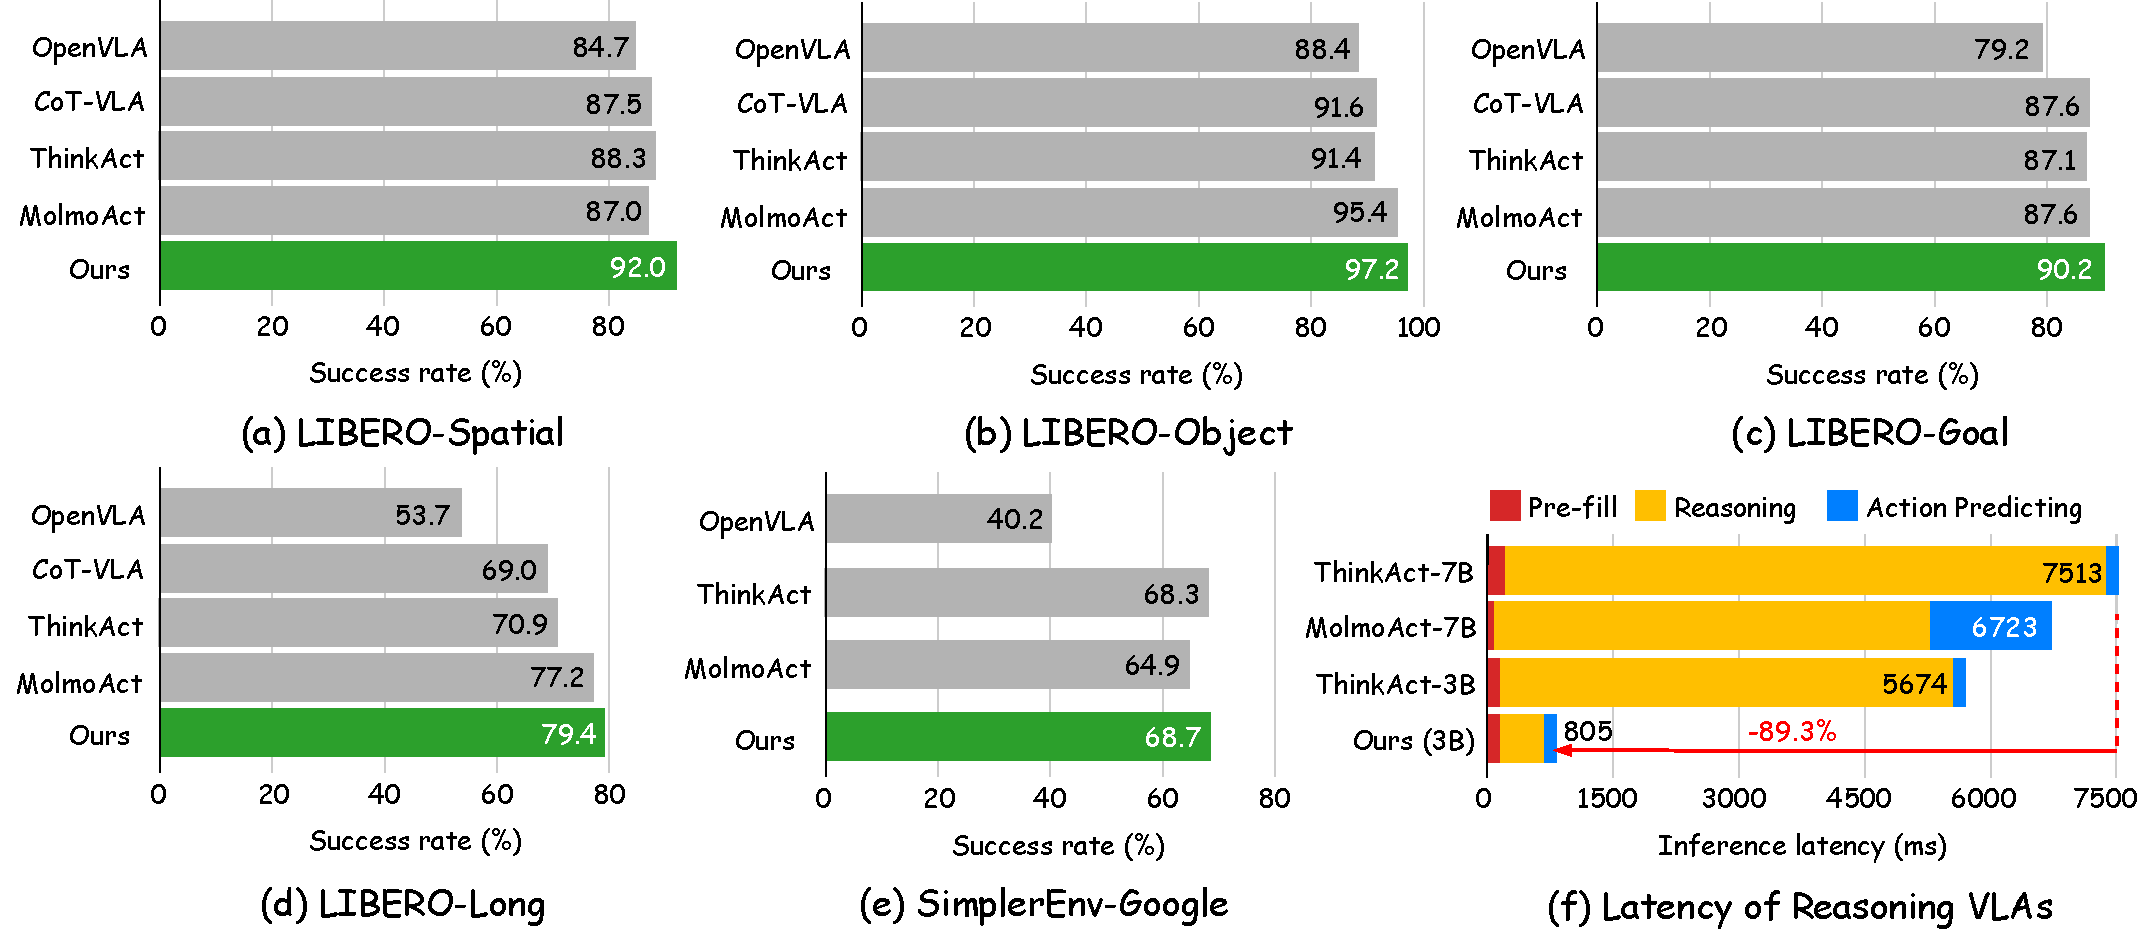
\includegraphics[width=1.0\linewidth]{figures/images/libero_simpler.pdf}
    \caption{\textbf{Evaluation of robot manipulation and reasoning efficiency.} (a)-(e) Success rates on LIBERO~\cite{liu2023libero} and SimplerEnv~\cite{li24simpler} benchmarks compared with state-of-the-art 7B reasoning VLAs. (f) Latency comparison across 3B and 7B reasoning VLAs. Our approach achieves up to 89.3\% inference latency reduction while maintaining superior task success rates.}
    \label{fig:libero_simpler}
    % \vspace{-3mm}
\end{figure*}


\subsection{Learning Strategy and Inference}\label{ssec:inference}

\noindent\textbf{Training Strategy.}
We initialize both teacher $\mathcal{F}_\theta^T$ and student $\mathcal{F}_\theta$ from the same checkpoint obtained through SFT and CoT-SFT on a pre-trained VLM. The teacher is trained with GRPO using action-aligned rewards~\cite{huang2025thinkact}, while the student is trained with $\mathcal{L}_\text{student}$ to compress reasoning into compact latents. We then connect the trained $\mathcal{F}_\theta$ with action model $\pi_\phi$ (initialized from~\cite{liu2024rdt}) by freezing $\mathcal{F}_\theta$ and the state encoder while updating the latent projector and $\pi_\phi$ with $\mathcal{L}_{\text{IL}}$ on large-scale robotic data. For target environment adaptation (e.g., LIBERO~\cite{liu2023libero}, RoboTwin2.0~\cite{chen2025robotwin2}), we fine-tune on environment-specific demonstrations.


\noindent\textbf{Inference.} 
The $\mathcal{F}_\theta$ processes $(o_t, l)$ by compact latent reasoning, generating visual trajectories via $K$ spatial tokens. The visual latent planning $c_t$, extracted from the spatial tokens' KV cache, conditions $\pi_\phi$ to predict actions $a_t$. Inference requires only $\mathcal{F}_\theta$ and $\pi_\phi$; the verbalizer $\mathcal{V}_\psi$ is used solely during training and optionally for interpretability.